\section{Simulation results}

The validation run uses the second-order design with \(T=\SI{2}{ms}\).
Table~\ref{tab:second-order-validated-estimates} shows that all four
parameters converge to their true ZOH values. In the window
\(t=\SIrange{3}{4}{s}\), all four parameters lie within
\(\SI{0.65}{\percent}\) relative error of their true ZOH values.

\begin{scripttable}
  \centering
  \caption{Validated second-order parameter estimates at \(T=\SI{2}{ms}\).}
  \label{tab:second-order-validated-estimates}
  \begin{tabular}{lrrr}
    \toprule
    Parameter & Estimated, \(t=\SIrange{3}{4}{s}\) & True & Absolute error \\
    \midrule
    \(a_1\) & \(-1.131310\) & \(-1.132176\) & \(8.66\times10^{-4}\) \\
    \(a_0\) & \( 0.134337\) & \( 0.135200\) & \(8.63\times10^{-4}\) \\
    \(b_1\) & \( 0.028348\) & \( 0.028362\) & \(1.49\times10^{-5}\) \\
    \(b_0\) & \( 0.014889\) & \( 0.014832\) & \(5.71\times10^{-5}\) \\
    \bottomrule
  \end{tabular}
\end{scripttable}

The static closed-loop gain is \(T(1)=1.000\). For the step at
\(t=\SI{5.5}{s}\), the response has no overshoot and the \(2\%\) settling time
is \(\SI{0.384}{s}\). The trace of \(P\) remains bounded at 400.
Figure~\ref{fig:second-order-simulation} shows the output, command, parameter
estimates, and covariance trace from this validation run.

\begin{figure}[htbp]
  \centering
  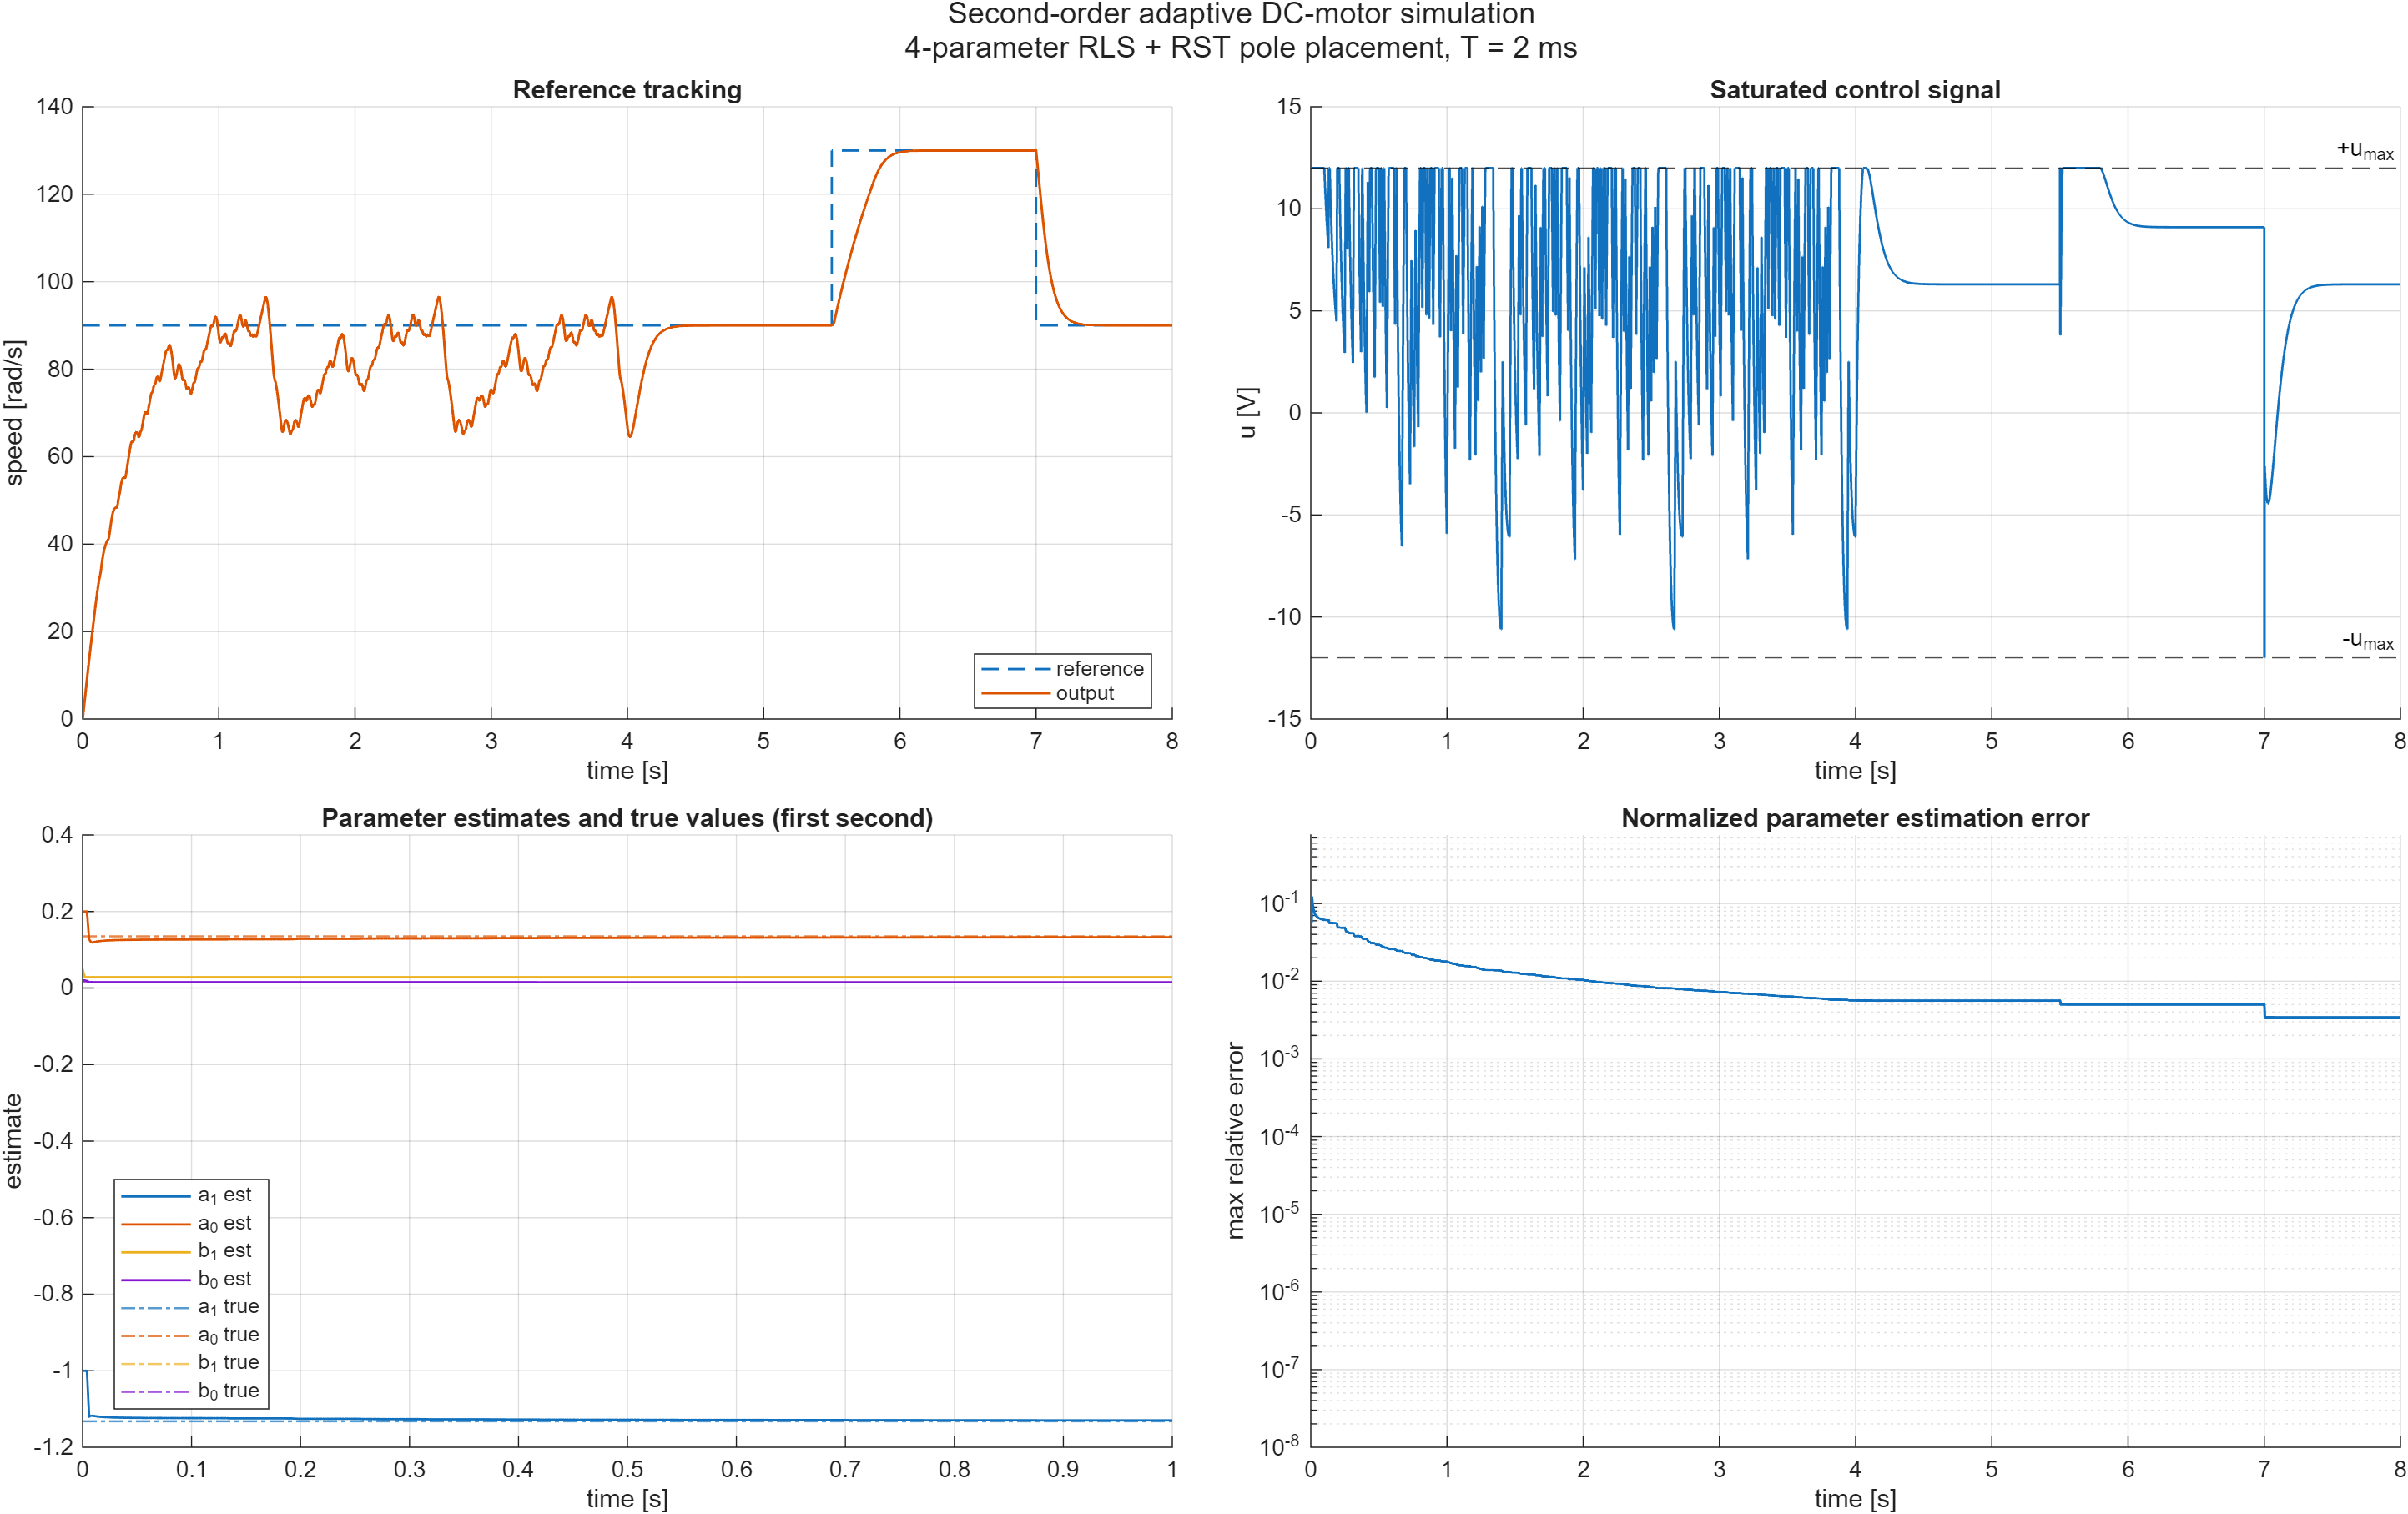
\includegraphics[width=0.62\linewidth]{../img/simulation_2nd_order.png}
  \caption{Validation run of the second-order adaptive RST controller.}
  \label{fig:second-order-simulation}
\end{figure}
